\chapter{Quase Eficiência}
\label{cap:grossman}

Sanford J. Grossman e Joseph E. Stiglitz, \citeonline{Grossman1980}, mostraram que é impossível para um mercado ser perfeitamente eficiente em termos de informação. Como as informações são dispendiosas, os preços não podem refletir perfeitamente as informações disponíveis, pois, se o fizessem, os investidores que gastassem recursos na obtenção e na análise não receberiam remuneração. Assim, um modelo sensato de equilíbrio de mercado deve deixar algum incentivo para a coleta de informações. Nas palavras dos autores os mercados devem apresentar "oportunidades de lucro suficientes, ou seja, ineficiências, para compensar os investidores pelo custo de negociação e coleta de informações."

Apenas no caso extremo e irreal, onde todas as informações e custos de negociação são zero, seria de se esperar que os preços refletissem totalmente todas as informações disponíveis. Mas se a informação é, de fato, sem custo, ela seria conhecida mesmo antes de os preços de mercado serem estabelecidos.

Como Fama reconheceu uma versão mais fraca e economicamente mais sensata de hipótese de eficiência seria necessária, ou seja, “os preços refletem as informações ao ponto em que os benefícios marginais de agir sobre a informação (os lucros a serem feitos) não excedem os custos marginais". Isso, por sua vez, torna a tarefa de testar a eficiência do mercado ainda mais complicada e exigiria modelos de precificação de ativos em equilíbrio que permitissem informações e custos de negociação em mercados com muitos agentes diferentes e com crenças não convergentes.

Diante dessas dificuldades, alguns defensores da HME optaram por uma noção baseada no comércio e definiram os mercados como eficientes, se não fosse possível para os investidores "obter retornos acima da média sem aceitar riscos acima da média", \citeonline{Malkiel2003}. Essa noção pode levar em conta informações e custos de transação e não envolve testar hipóteses conjuntas. Mas isso está muito distante da ideia básica de mercados como alocadores eficientes de capital entre países, indústrias e empresas.

Possibilidade de vencer o mercado como um teste de eficiência deste também apresenta novos desafios. Embora seja certamente possível construir estratégias de negociação (inclusive com custos de transação) com índices de Sharpe que excedam aquele da carteira de mercado, \emph{ex-post}, é improvável que tais evidências sejam convincentes para os defensores da HME. Pode-se argumentar que elas são realizadas com o benefício da retrospectiva, e é improvável que sejam repetidas em tempo real. Diante desta nova definição de eficiência e dos testes sugeridos, as seguintes considerações devem ser levadas em conta:

\begin{itemize}
	\item Mineração de dados
	\item Mudanças estruturais e instabilidade dos modelos
	\item Relações positivas que existem entre custos de transação e previsibilidade de retornos
	\item Volatilidade do mercado e aprendizagem
\end{itemize}

O teste de "bater o mercado" também não ajuda a descobrir a natureza e extensão das ineficiências. Um teste com abordagem estrutural seria desejável. Uma das formas de testar a eficiência de mercado neste novo paradigma é através de estudos de eventos, onde um evento que pode ser perfeitamente datado é analisado em vistas de seu impacto no preço do ativo. Um mercado eficiente (ou quase eficiente na presença de custos) deve precificar rapidamente a nova informação, havendo ainda algum \emph{drift} nos preços em função justamente dos custos friccionais.

Há uma grande literatura de estudo de eventos sobre questões em finanças corporativas. Os resultados indicam que, em média, os preços das ações se ajustam rapidamente a informações sobre decisões de investimento, mudanças de dividendos, mudanças na estrutura de capital e transações de controle corporativo. Essa evidência nos leva a crer que os preços se ajustam de maneira eficiente às informações específicas da empresa. Mais importante, a pesquisa revela regularidades empíricas, muitas delas surpreendentes.

Uma descoberta interessante é que mudanças inesperadas nos dividendos são, em média, associadas a mudanças de mesmo sinal nos preços das ações. O resultado é uma surpresa, dado que o teorema de Miller-Modigliani prediz que a política de dividendos é irrelevante ou que os dividendos são más notícias porque, durante os períodos dos testes, os dividendos são tributados a uma taxa maior do que os ganhos de capital. A evidência sobre a resposta dos preços das ações às mudanças de dividendos leva a modelos de sinalização  e teorias de fluxo de caixa livre que tentam explicar por que os aumentos de dividendos são boas notícias para os preços das ações. 

\citeonline{Foster1984}, examinaram o impacto dos anúncios de lucros nos retornos das ações. Cada anúncio de resultados para uma grande amostra de empresas foi colocado em decis classificados 1 de 10 pela magnitude da surpresa dos lucros, e os retornos anormais das ações em cada decil foram calculados. O retorno anormal em um período é o retorno de uma carteira de todas as ações em um determinado decil após o ajuste para o retorno de mercado nesse período e para o beta do portfólio. Ele mede o retorno acima do que seria esperado dadas as condições de mercado naquele período. A figura \ref{fig:figgrosreturns} é um gráfico dos retornos anormais cumulativos para cada decil.

\begin{figure}[h]
	\centering
	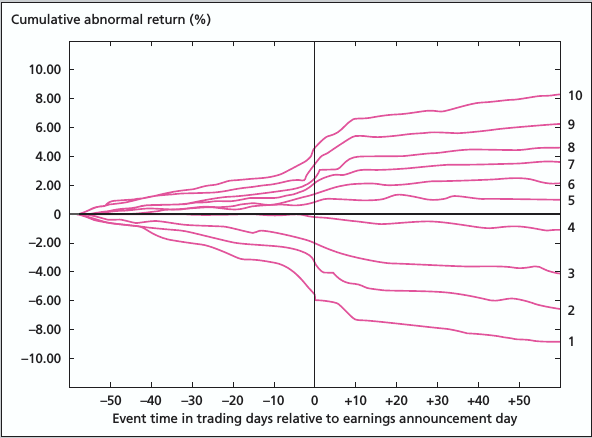
\includegraphics[width=1\linewidth]{figs/fig_gros_returns}
	\caption[Retornos anormais após anúncios de lucros.]{Retornos anormais acumulados após anúncios de lucros.\\ Fonte: Foster (1984).}
	\label{fig:figgrosreturns}
\end{figure}

O resultado mais interessante do estudo diz respeito aos movimentos dos preços das ações após a data do anúncio. Os retornos anormais acumulados de ações com surpresa positiva continuam a crescer mesmo depois do anúncio de lucros se tornar público, enquanto as empresas com surpresa negativa continuam a sofrer retornos anormais negativos. O mercado parece se ajustar às informações de ganhos apenas gradualmente, resultando em um período sustentado de retornos anormais. Desta forma, seria possível obter lucros anormais simplesmente esperando por anúncios de ganhos e comprando uma carteira de ações de empresas com lucros anunciados acima dos previstos. Esses são precisamente os tipos de tendências  previsíveis que deveriam ser impossíveis em um mercado eficiente.

Algumas pesquisas sugerem que o desvio pós-anúncio nos preços de ações pode estar relacionado aos custos de negociação. Eles também apontam que retornos anormais pós-anúncio são maiores para empresas menores, para as quais os custos de negociação são mais elevados. Ainda assim, esses resultados não explicam totalmente esta anomalia. Embora os custos de negociação possam explicar a existência de desvios após os anúncios, eles não explicam por que o retorno anormal total é maior para empresas com maiores surpresas de lucros.

\section{Ineficiência versus Prêmio de Risco}

Como devem ser interpretados todos estes estudos que sugerem grandes ineficiências no mercado? Simples regras para formação de portfólios que batem o mercado, são ineficiências ou os retornos em excesso são resultado de prêmios recebidos pelo risco maior incorrido? Em todas estas estratégias que rendem lucros aumentados, caso o risco inerente a estas também seja mais alto, o investidor está apenas recebendo seu justo retorno ajustado ao risco e não verdadeiramente um lucro anormal, e portanto estaria de acordo com a atual hipótese de eficiência dos mercados.

\citeonline{Fama1993} argumentam que essas anomalias podem ser explicadas como manifestações de prêmios de risco. Utilizando uma abordagem de precificação de equilíbrio por arbitragem eles mostram que ações com maior sensibilidade aos fatores tamanho ou patrimônio/preço têm retornos médios mais altos e interpretam esses retornos como evidência de um prêmio de risco associado a esses fatores. Fama e French argumentam que o chamado modelo de três fatores, em que o risco é determinado pela sensibilidade de uma ação para: (1) a carteira de mercado (beta de mercado), (2) uma carteira que reflete os retornos relativos de pequenas e grandes empresas e, (3) um portfólio que reflita os retornos relativos de empresas com índices altos versus baixos de valor contábil (patrimônio) sobre preço, faz um bom trabalho ao explicar os retornos de ativos. Embora os índices de tamanho ou de patrimônio/preço, por si só, não sejam fatores de risco, talvez possam servir como \emph{proxies} para determinantes mais fundamentais do risco. Fama e French argumentam que esses padrões de retorno podem, portanto, ser consistentes com um mercado eficiente, no qual os retornos esperados são consistentes com o risco.

Uma interpretação oposta é oferecida por \citeonline{Lakonishok1994}, que argumentam que esses fenômenos são evidências de mercados ineficientes, mais especificamente, de erros sistemáticos nas previsões dos analistas do mercado de ações. Eles apresentam evidências de que os analistas extrapolam o desempenho passado muito para o futuro e, portanto, superestimam empresas com desempenho recentes bons e subprecificam aquelas com desempenho recente ruim.
